\section{Implementation and Performance Assessment}\label{sec:exp}

\begin{figure}
\centering
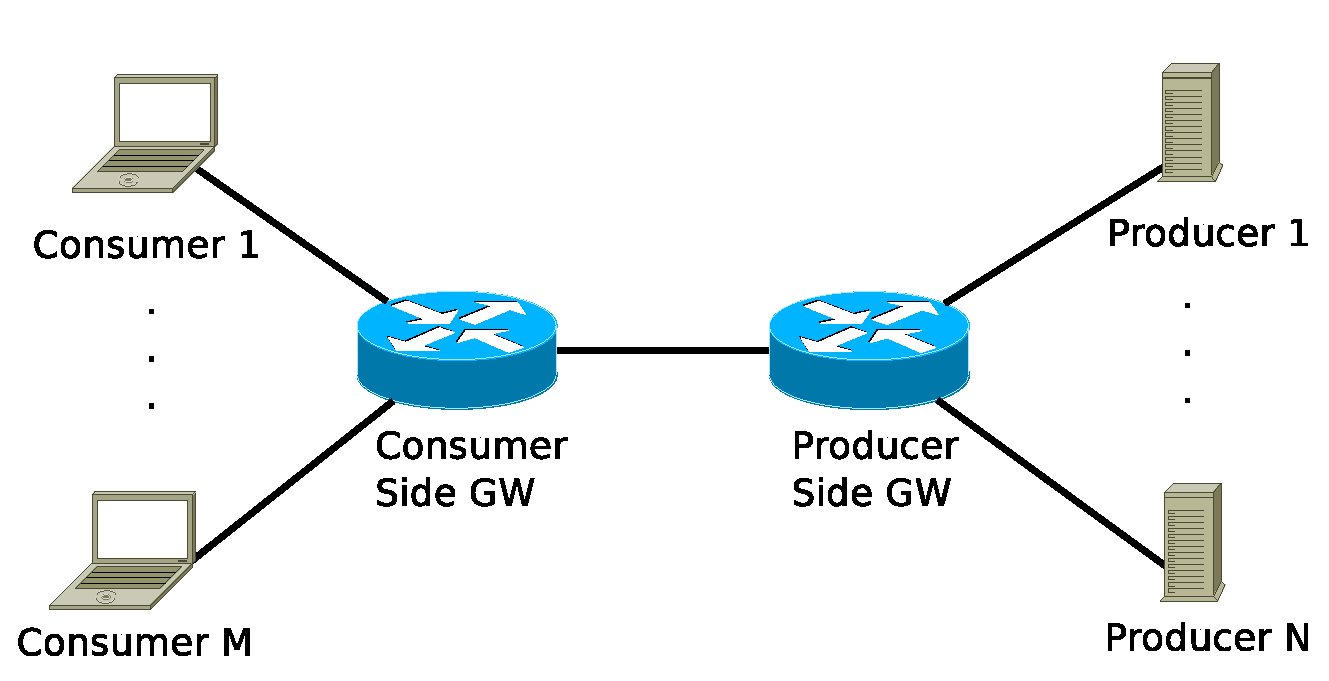
\includegraphics[width=\columnwidth]{images/testnet.eps}
\caption{Testbed network topology. $M$ consumers and $N$ producers}\label{testnet}
\end{figure}

\begin{figure}
\centering
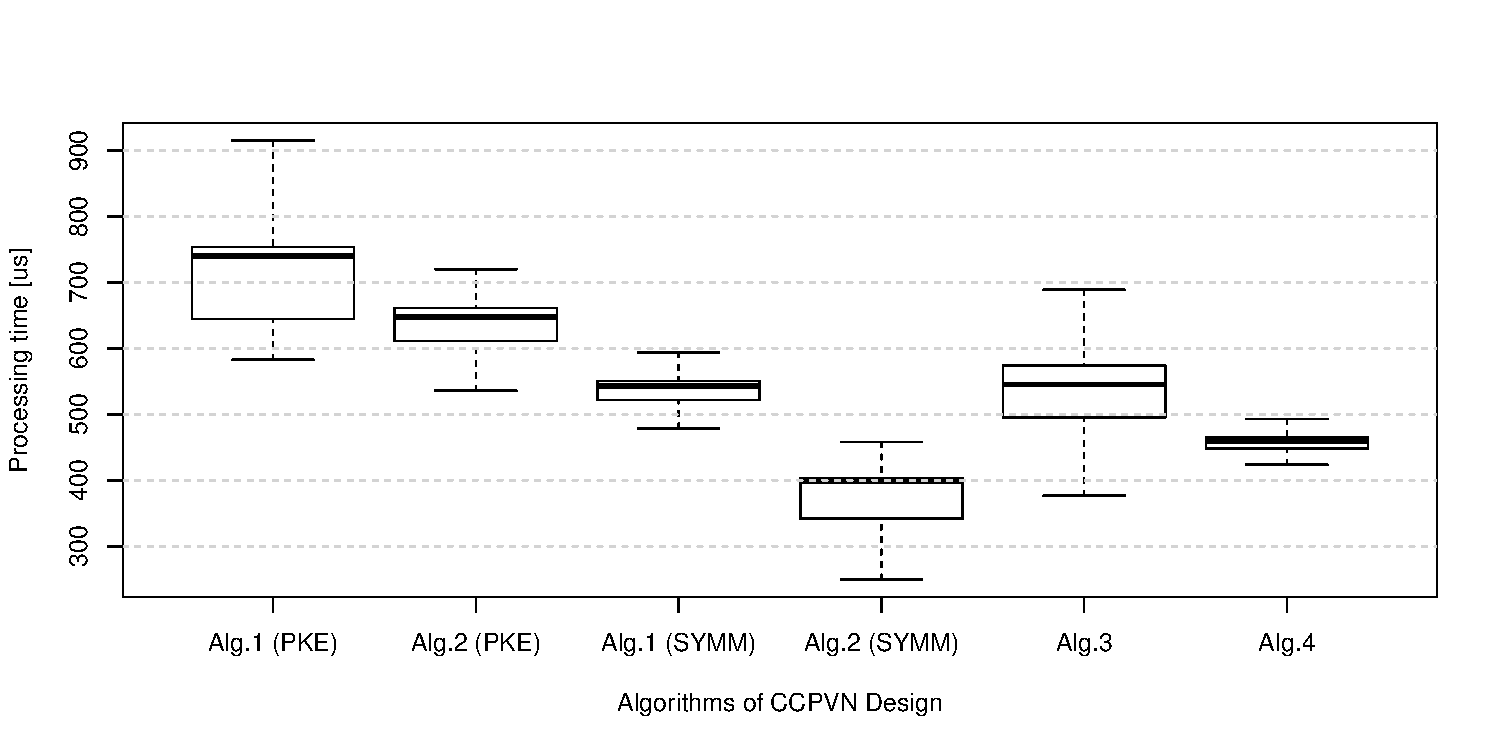
\includegraphics[width=\columnwidth]{images/times.pdf}
\caption{Execution time of the algorithms in CCVPN design}\label{times}
\end{figure}

\begin{figure}
\centering
  \subfigure[Throughput]{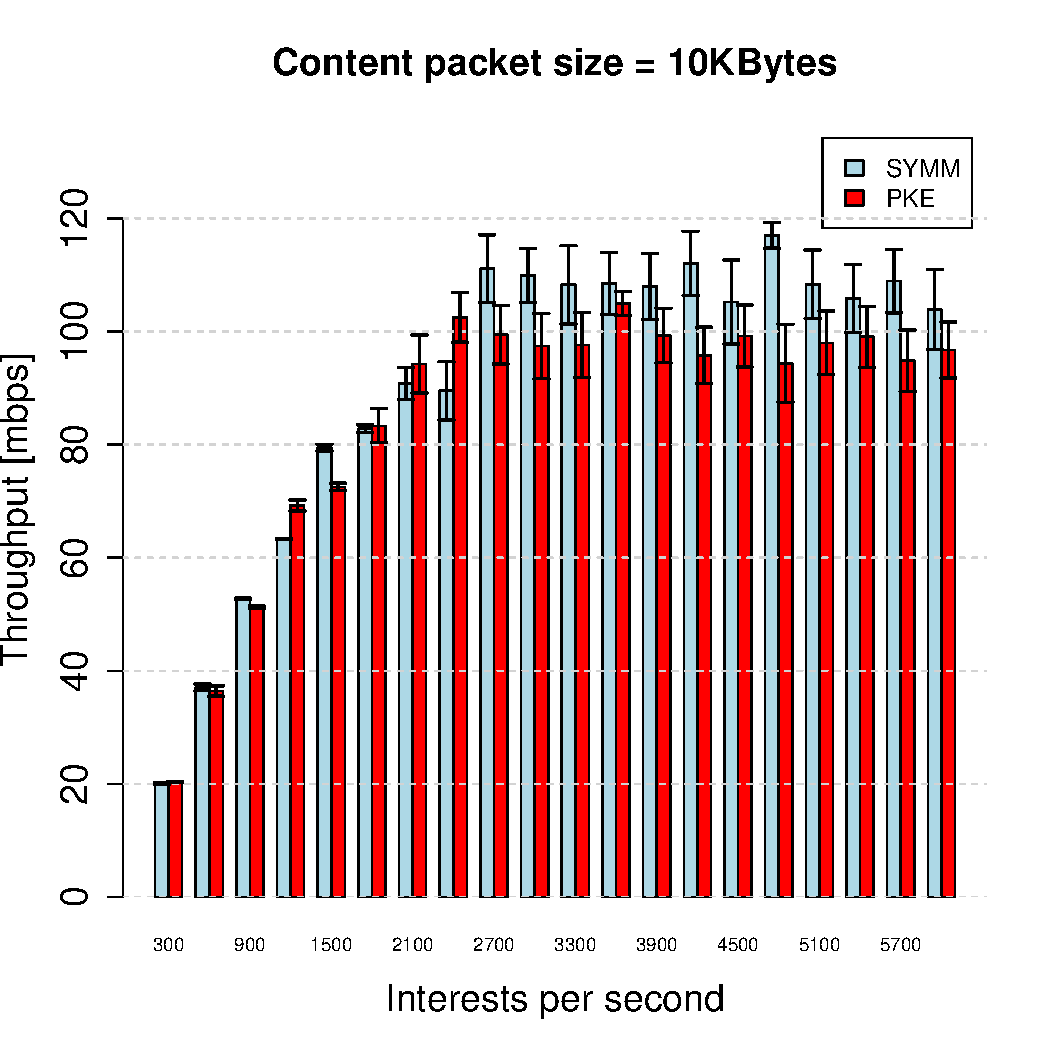
\includegraphics[width=0.8\columnwidth]{images/1_1_thput.pdf}\label{1a}}
  \hfil
  \subfigure[Avg. RTT]{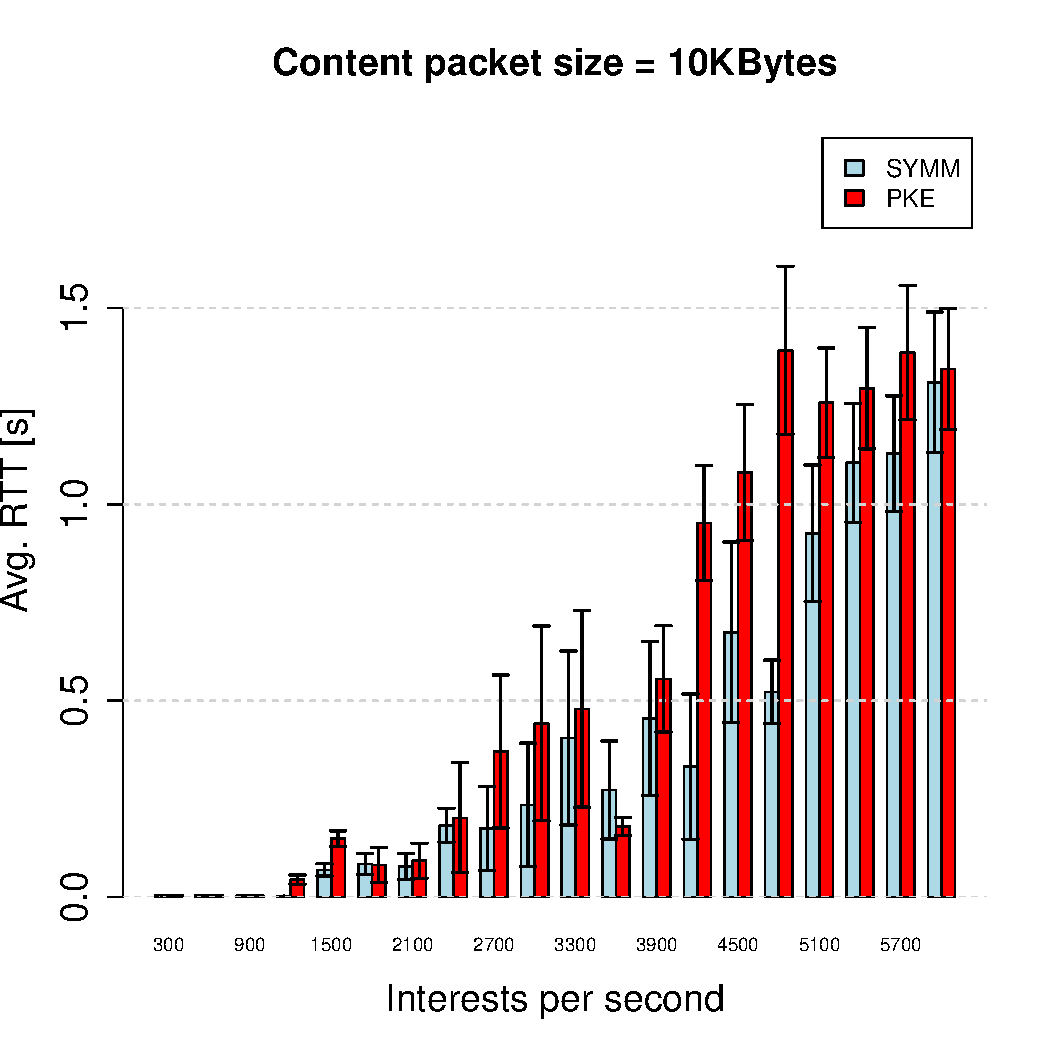
\includegraphics[width=0.8\columnwidth]{images/1_1_rtt.pdf}\label{1b}}
\caption{CCVPN performance with one consumer and one producer for increasing interest issuance rates.}\label{exp1}
\end{figure}

\begin{figure}
\centering
  \subfigure[Throughput]{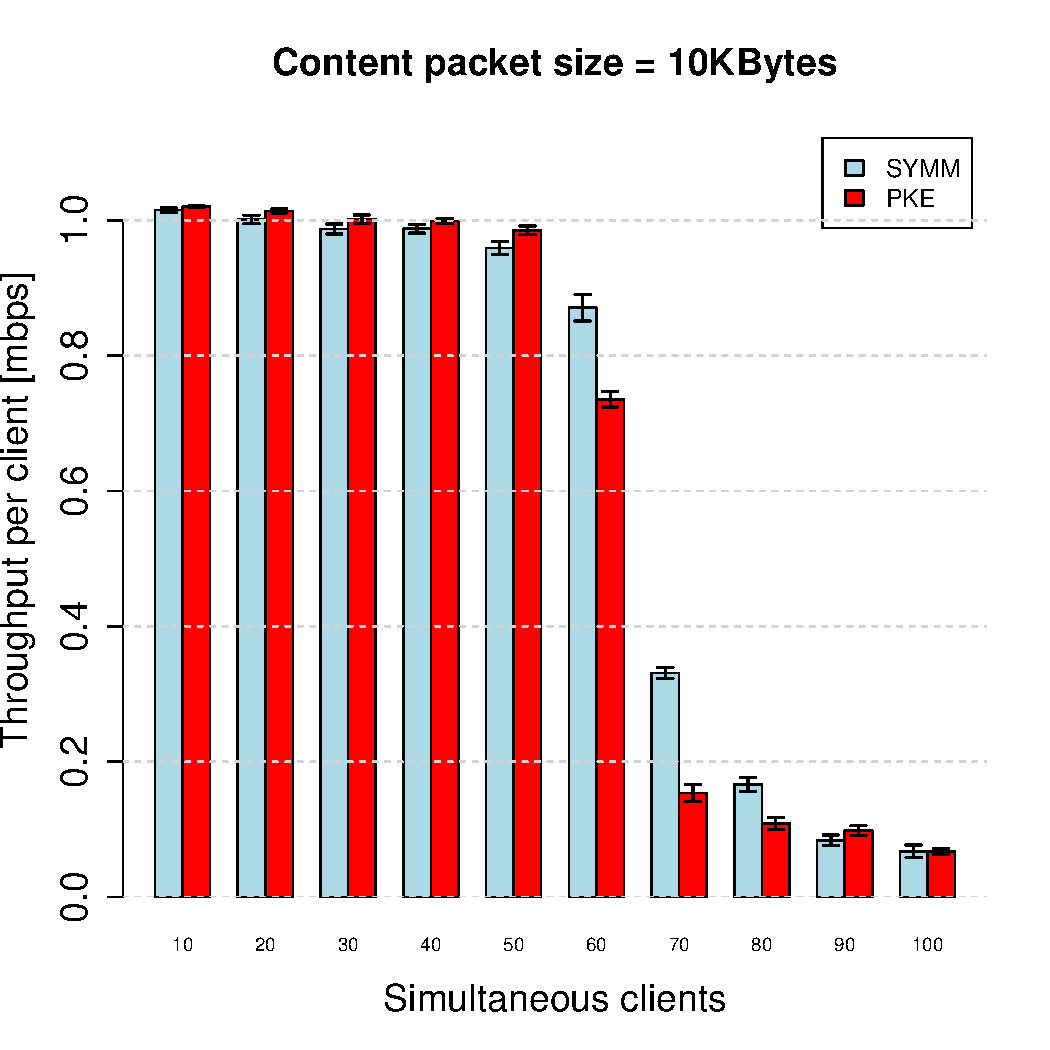
\includegraphics[width=0.7\columnwidth]{images/n_1_thput.pdf}\label{2a}}
  \hfil
  \subfigure[Avg. RTT]{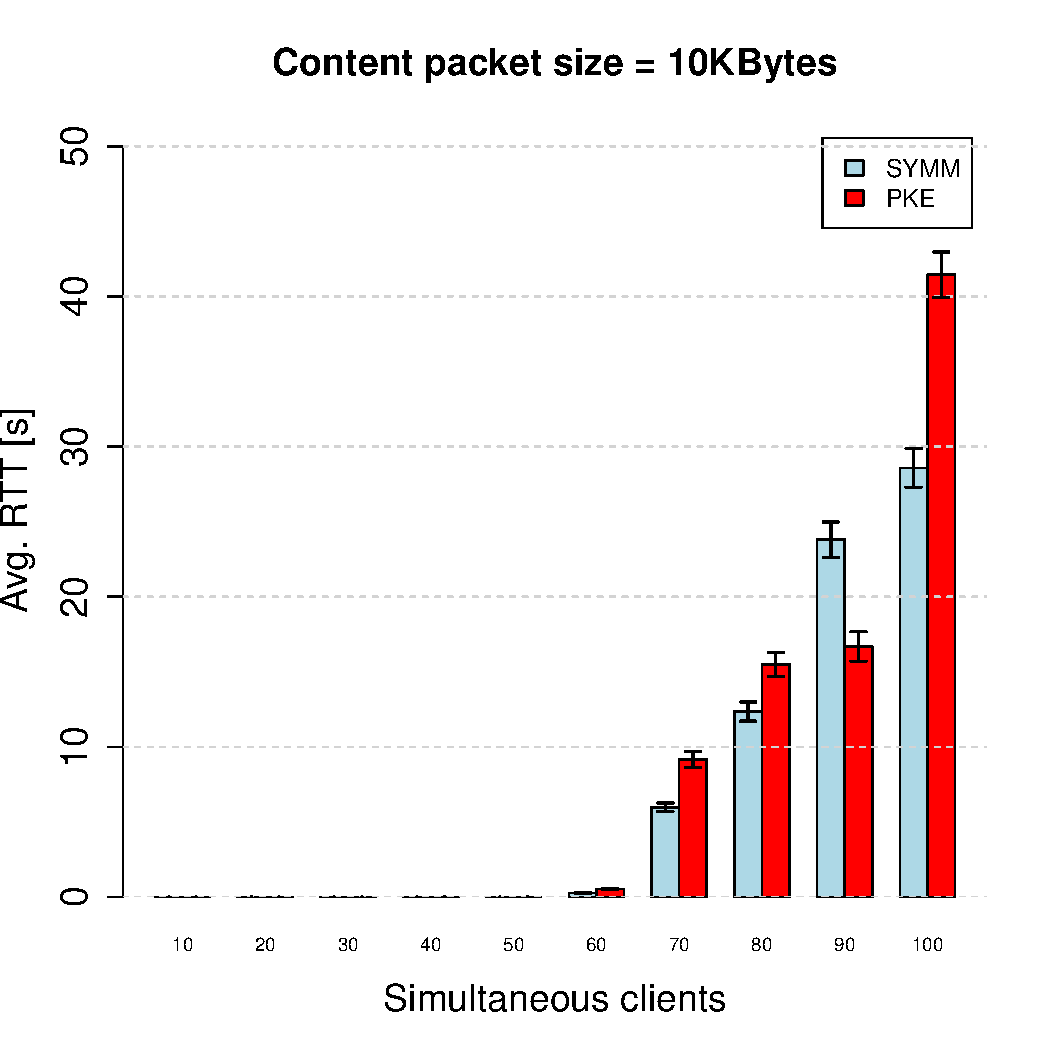
\includegraphics[width=0.7\columnwidth]{images/n_1_rtt.pdf}\label{2b}}
\caption{CCVPN performance with multiple consumers and one producer. Each consumer requests with 1 mbps rate.}\label{exp2}
\end{figure}

\begin{figure}
\centering
  \subfigure[Throughput]{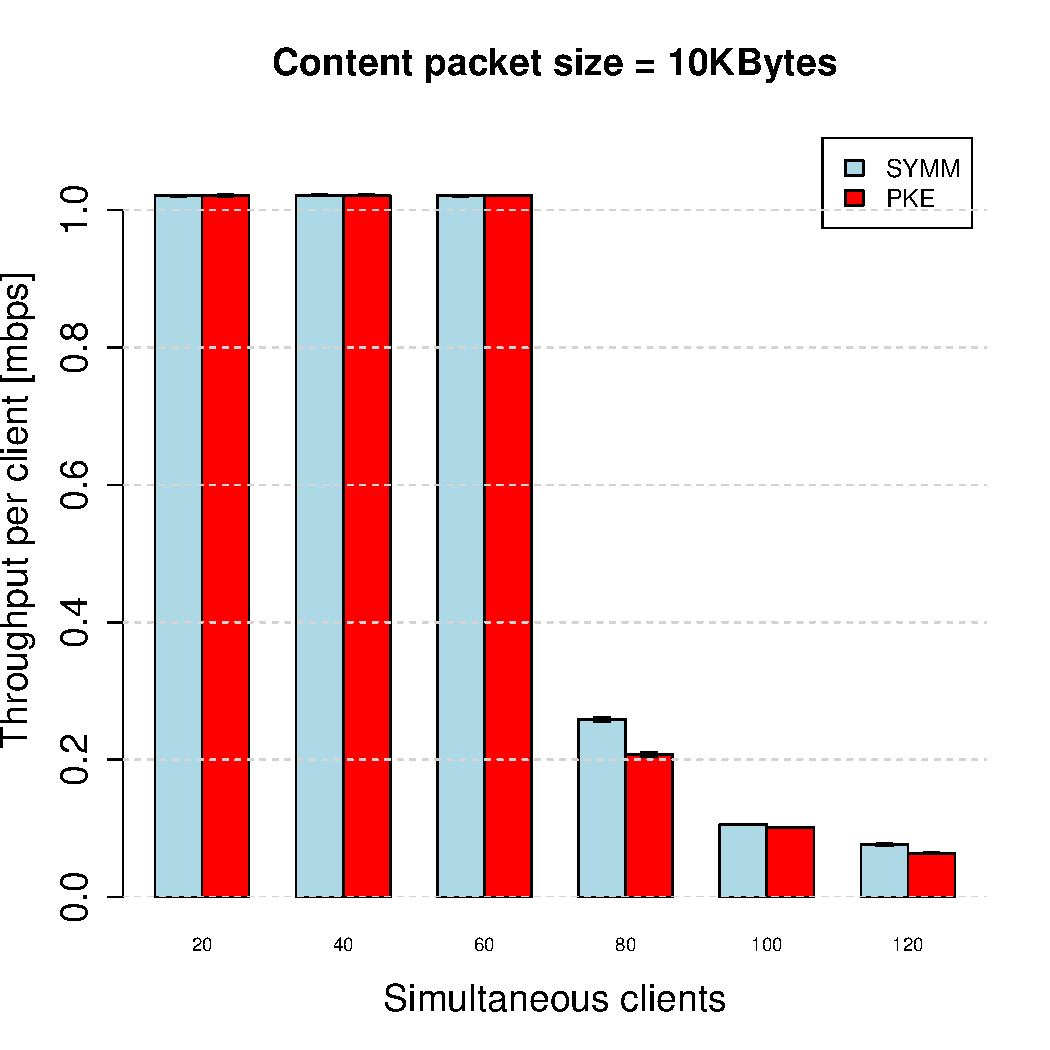
\includegraphics[width=0.7\columnwidth]{images/n_n_thput.pdf}\label{3a}}
  \hfil
  \subfigure[Avg. RTT]{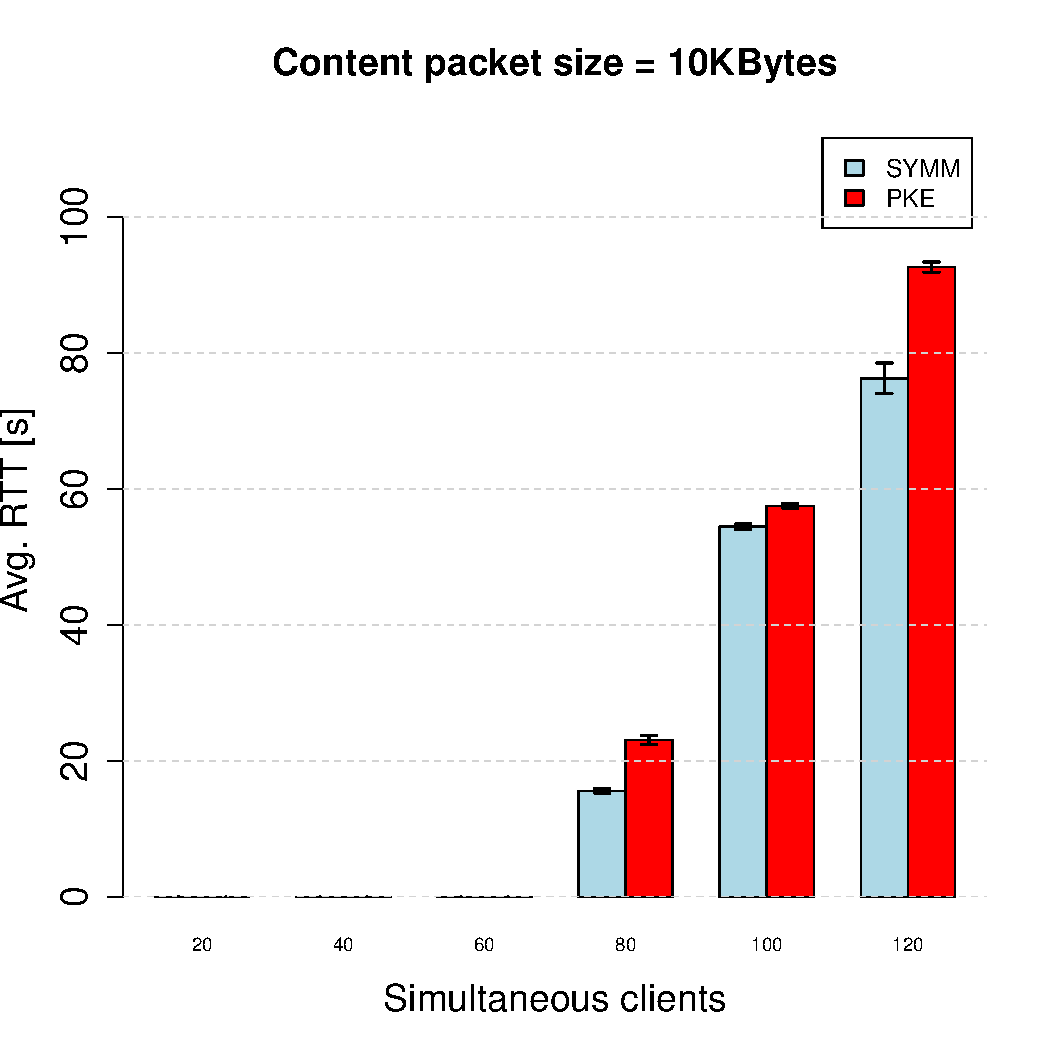
\includegraphics[width=0.7\columnwidth]{images/n_n_rtt.pdf}\label{3b}}
\caption{CCVPN performance with multiple consumers and multiple producers. Each consumer requests with 1 mbps rate.}\label{exp3}
\end{figure}


CCVPN is implemented as a network layer service running on the gateways of the private networks that compose the VPN (see Fig.\ref{fig:ccvpn}).
Our implementation uses the CCNx software stack~\cite{CCNxGithub} and the cryptographic library Sodium~\cite{sodiumGithub}. These are both publicly available and written in C.
For the PKE version of CCVPN, we use Sodium Sealed-Boxes~\cite{bernstein2006curve25519}, implemented over X25519 elliptic curves, as the PKE algorithm for the interest encapsulation and decapsulation routines (Algorithm~\ref{alg:interestEncap}, and Algorithm~\ref{alg:interestDecap} of Sec.~\ref{metho}).
AES256-GCM~\cite{dworkin2007recommendation} is used to encrypt-then-MAC content responses (Alg.~\ref{alg:contentEnc}, and Alg.~\ref{alg:contentDec} of Sec.~\ref{metho}).
Recall that the symmetric keys used to encrypt-then-MAC the content packets are generated and sent together with the encapsulated interest in Alg.~\ref{alg:interestEncap}.
In the symmetric key version of the design, both, interests and contents, are encapsulated using AES256-GCM under the assumption that the gateways already share a symmetric key.


The experiments presented throughout this section were executed in an Intel Core i7-3770 octacore CPU @3.40GHz, with 16GB of RAM, running Linux (Ubuntu 14.04LTS). Content payload sizes were set to 10 kilobytes.
On every experiment, each of the two gateway processes (i.e., consumer side gateway process, and producer side gateway process) were assigned as a high priority processes and each of them ran in a single core of the processor.
Fig.~\ref{times} presents box-plots for the execution times of the four algorithms involved in CCVPN's data transmission, including both, PKE and Symmetric Key versions for interest encapsulation and decapsulation.

With the goal of evaluating the impact of CCVPN's cryptographic overhead on the overall network performance, we measure the network throughput and the request-response round trip time (RTT) under different topology settings.
In our testbed network, the consumers' side and the producers' side gateways are directly interconnected. $N$ producers are connected to the producers' domain gateway and $M$ consumers are connected to the consumers' domain gateway, as illustrated in Fig.~\ref{testnet}.
In this topology, we consider three variations for the values of ${M,N}$:

\begin{itemize}
 \item \textbf{One consumer and one producer $[1,1]$}: We use this setting, with only one consumer and one producer, to slowly increase the interest issuance rate until we are able to determine the maximum network throughput and the impact on RTT as congestion increases.
 \item \textbf{Multiple consumers and one producer $[M,1]$}: In this setting we fix the interest issuance rate so that each consumer requests approximately 1 mbps of data, and we gradually increase the number of consumers in the network, until the throughput per consumer starts to decrease, i.e., until congestion starts to occur. In this setting, the interests coming from all consumers are served by a single producer.  
 \item \textbf{Multiple consumers and multiple producers $[M,N]$}: In this experiment we also gradually increase the number consumers, but we increase the number of producers by the same amount at each round, i.e., $M=N$. The number of hosts (consumers and producers) is increased until congestion is observed.
\end{itemize}

It is worth to mention that, in all of the considered settings, every interest is a unique request for a unique piece of content. Therefore, the experiments present the throughput and RTT in the worst case scenario of a CCN, i.e., when there is no content caching in the gateway.

Fig.~\ref{exp1} shows the the network performance when $[M,N]=[1,1]$ as the consumer's request rate increases. The network achieves a maximum throughput of 100 mbps in the PKE version and a
slightly higher throughput of 110 mbps in the symmetric key version. Conversely, the average RTT per message starts to increase as the interest issuance rate approaches the maximum network throughput, as a signal of congestion in the routers.

The results for multiple consumers requesting to a single producer ($[M,1]$) are depicted in Fig.~\ref{exp2}.
In this setting, each consumer receives close to the requested throughput (1 mbps) when less than 50 clients are requesting contents at the same time.
With more than 60 clients the Avg. RTT starts to increase due to congestion, and the average throughput experienced by each client is gradually reduced.

Since in CCN the consumer signs every content, the congestion presented in Fig.~\ref{exp2} might be influenced by the overhead of having a single producer signing an enormous number of interests, in addition to the gateways' cryptographic overhead.
To evaluate that effect in Fig.~\ref{exp3}, we show the average throughput and RTT in the scenario with $[M,N]$ consumers and producers, where $M=N$ and each consumer requests from a specific producer.
In such scenario, we see that the results are slightly better. The network offers the requested throughput (1 mbps per client) with up to 60 nodes, in PKE mode, and 70 nodes, in symmetric key mode.


\subsection{Discussion}

CCVPN  exhibits moderately good results with respect to the network load capacity, considering the overheads implied by the deployment of secure tunnels over the CCN architecture.
With gateways' processes running each on a single core of a single processor, the VPN was capable of providing reasonable throughput to up to 70 clients.
This performance results are a lower bound that can be improved in several ways, among which we highlight:

\begin{enumerate}
 \item \textbf{Implementation optimization:} The CCNx software stack is an ongoing research project, and as such, the implementation focus on functionality rather than performance.
 We believe that the results presented in this section could be significantly improved by optimizations that do not rely exclusively on CCVPN design, but also in CCNx software.
 \item \textbf{Distributed and parallel processing:} In a real deployment scenario, we expect that a large scale organization, which wants to implement a VPN service, to have dedicated network devices running
 the gateway service, possibly in multiple cores. Moreover, it is not hard to imagine multiple VPN gateways sharing the load in a large organization.
 In such scenarios, we expect the network capacity (in terms throughput or number of simultaneous consumers) to scale linearly with the increase of dedicated computational resources.
 \item \textbf{Caching:} Content caching is a major advantage of ICNs when compared to the IP model. In our experiments we wanted to evaluate the worst case scenario. Therefore, clients always request different contents
 and content caching does not happen. In a real world deployment, contents that are popular (inside the VPN) would be potentially cached, significantly increasing the throughput and reducing the RTT.
 
\end{enumerate}



